% This is my first .tex document. It's used to learn LateX while writing my end of studies report.

%----------------------------------------------------------------------------------------
%	PACKAGES AND OTHER DOCUMENT CONFIGURATIONS
%----------------------------------------------------------------------------------------
\documentclass[11pt]{article}
\usepackage[english, french]{babel}
\usepackage[utf8]{inputenc}
\usepackage{graphicx}
% Used to format pars, specify the indent size and jump after par ending
\usepackage[skip=10pt plus1pt, indent=25pt]{parskip}

% Used to allow n-depth level for titles (pars become numbered). 
\usepackage{titlesec}
\setcounter{secnumdepth}{5}

% Hyphenation for languages with accented characters 
% is the main reason that requires T1 font encoding.
\usepackage[T1]{fontenc}

% Used to manage hyperlinks and make a clickable table of contents.
\usepackage{hyperref}
\hypersetup{
    colorlinks,
    citecolor=blue,
    filecolor=red,
    linkcolor=black,
    urlcolor=green
}

% Defines graphics path.
\graphicspath{ {./images/} }

% Defines a new command for the horizontal lines, change thickness here.
\newcommand{\HRule}{\rule{\linewidth}{0.5mm}} 

\begin{document}

  \begin{titlepage}   
    % Center everything on the page.
    \center 

    %----------------------------------------------------------------------------------------
    %	LOGO SECTION
    %----------------------------------------------------------------------------------------

    \begin{figure}[!tbp]
      \centering
      \begin{minipage}[t]{0.4\textwidth}
        
\includegraphics[width=\textwidth]{Logo_ESIEA.jpg}    
      \end{minipage}
      % \hfill is used to evenly distribute the logos
      \hfill 
      \begin{minipage}[t]{0.4\textwidth}
        
\includegraphics[width=\textwidth]{Logo_Aubay.jpg}    
      \end{minipage}
    \end{figure}

    %----------------------------------------------------------------------------------------
    %	TITLE SECTION
    %----------------------------------------------------------------------------------------

    % Black horizontal line.
    \HRule \\[0.4cm]
  
    { \huge \bfseries Mission de fin d’études}\\ 
    % Space below "Mission de fin d'étude.
    \vspace{5ex}
    { \huge \bfseries Find Your Way}
    
    \HRule \\[0.8cm]
    \textsc{\LARGE Aubay}\\[1.5cm]
    
    %----------------------------------------------------------------------------------------
    %	AUTHOR SECTION
    %----------------------------------------------------------------------------------------

    \begin{minipage}{0.4\textwidth}
      \begin{flushleft} \large
        \emph{Maître de stage:} \\
        Nathan  \textsc{CANTAT} 
      \end{flushleft}
    \end{minipage}
    ~
    \begin{minipage}{0.4\textwidth}
      \begin{flushright} \large
        \emph{Jury de stage:} \\
        Arnaud  \textsc{BANNIER} 
      \end{flushright}
    \end{minipage}\\[2cm]
    
    \begin{minipage}{0.4\textwidth}    
      \emph{Auteur:}\\
      \bfseries \Large Nicolas \textsc{Cisternas}      
    \end{minipage}\\[2cm]

    %----------------------------------------------------------------------------------------
    %	DATE SECTION
    %----------------------------------------------------------------------------------------

    \large 28 février - 31 août 2022

  \end{titlepage}

  % Used to write the abstract in french.
  \selectlanguage{french} 
  \begin{abstract}
    Vous donnerez une description du
    sujet et des grandes parties de l’ouvrage. Il s’agit ici de motiver un lecteur potentiel en lui
    décrivant le contenu du document et les implications que l’on peut en tirer,
  \end{abstract}
  \pagebreak

  % Used to write the abstract in english.
  \selectlanguage{english} 
  \begin{abstract}
    Abstract in English
  \end{abstract}
  \pagebreak

  \selectlanguage{french} 
  \setcounter{tocdepth}{5}
  \tableofcontents

  \pagebreak

  \section{Remerciements}    
    Je remercie Éric REMILLERET et Nathan CANTAT, mes maîtres de stage, 
    ainsi que Wael NASR, pour m'avoir donné l'opportunité de rejoindre 
    Aubay Innov', qui s'est avérée être une expérience intéressante 
    et instructive, ainsi que pour l'aide à la relecture de ce rapport.    
    
    Je remercie Anne-France GALLAND, qui a largement contribué à la phase de suivi et d'organisation du projet, par ses interventions 
    lors des réunions hebdomadaires et pour le temps qu'elle a pris pour la relecture de ce rapport.    
    
    Je remercie Jean-Philipe CUNNIET, mon tuteur de stage ainsi qu'Arnaud BANNIER, le jury de cette mission de fin d'études, 
    pour le temps qu'ils ont passé à relire et évaluer ce rapport de stage ainsi que la soutenance de stage.    

    Je tiens à remercier toute l'équipe avec laquelle j'ai 
    travaillé durant mon stage:    
    Nicolas GUILLERMAIN et Mathieu MONNERET avec qui j'ai travaillé lors 
    de la phase d'état de l'art et de preuve de concept.
    Mélissa WANG et Jeoffrey MENUDIER avec qui j'ai principalement 
    travaillé lors de la phase projet. 
    Jean-Baptiste CHANIER, Victor CHAVEROT, Jean-Noël CLINK,
    Ophélie PHONCHAREUN, Miora RASOLOFONERA et Rémi VIDAL avec qui j'ai échangé tout au 
    long du stage concernant leurs parties du projet.       
    
    Je tiens également à remercier la direction générale d'Aubay pour leur accueil et leur écoute ainsi qu'Ophélie CHEVALIER, campus manager, 
    pour tous les événements qu'elle a pu organiser et qui ont permis d'établir un climat chaleureux entre les différents groupes.
        
    Enfin, je remercie les autres étudiants d’Aubay Innov' avec lesquels j'ai eu l'occasion d'échanger aussi bien humainement que techniquement.

  \pagebreak
  \section{Introduction et contexte}    
  
  Mon stage s'est déroulé dans une entreprise appelée Aubay, pour une durée de 6 mois (du 28 février 2022 au 31 août 2022). 
  En détail, Aubay est une ESN (Entreprise de Services Numériques) qui a été fondée par Christian Aubert en 1998 et 
  dont le siège social est situé au 13 rue Louis Pasteur à Boulogne-Billancourt. L'entreprise est spécialisée dans les domaines 
  liés à la finance, à l'assurance et à la banque et est également impliquée dans divers marchés, tels que les télécoms, 
  les services, les réseaux, l'énergie et les transports. Aubay accompagne la transformation et la modernisation des systèmes 
  d’information de ses clients. Ils opèrent sur des marchés à forte valeur ajoutée, en France comme en Europe. C'est un acteur 
  référent de la transformation digitale. Son secteur d'activité est centré autour du conseil sur tout type de projet technologique.  
  C'est une ESN cotée en Bourse (SBF 250) et 46\% du capital est détenu par les managers. Les chiffres clés concernant Aubay 
  sont présentés dans la Figure \ref{fig:PA1} ci-après. En 2022, l'entreprise emploie 7306 travailleurs, dont 2728 en France. 
  Selon son site internet, Aubay est implanté dans 7 pays européens, et a réalisé un chiffre d'affaires de 470,6 M€ en 2021. 
  D'ailleurs, ces dernières années, l'entreprise a connu une forte croissance de 10,4\% en 2021, qui coïncide avec une augmentation 
  constante des effectifs de l'entreprise, passant de 4600 employés en 2015 à plus de 7000 aujourd'hui.
 
  \begin{figure}[hbt]  
    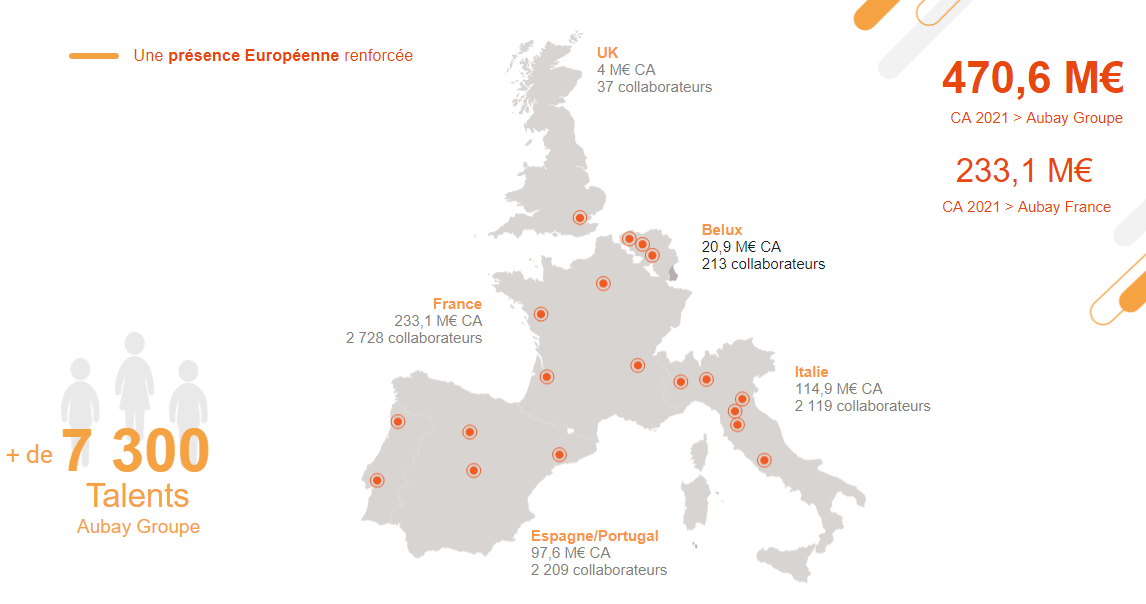
\includegraphics[width=\textwidth]{PresentationAubay1.png}    
    \caption{Chiffres clés pour Aubay en 2021.}
    \label{fig:PA1}
  \end{figure}  
  
  J'ai eu le privilège d'effectuer mon stage au sein de l'unité "Aubay Innov'" qui est la division d’Aubay France dédiée 
  à la recherche et à l'innovation. Ses membres sont impliqués dans différents projets, chacun lié à la data science, l'analyse 
  de données ou tout autre domaine liés aux nouvelles technologies numériques. L'objectif de l'unité est d'acquérir 
  les connaissances et le savoir-faire pour construire des solutions durables et innovantes adaptées aux besoins futurs des clients. 
  Les projets dirigés dans la cellule innovation d'Aubay ne sont donc soumis à aucun client pendant leur réalisation, 
  ce qui laisse l'opportunité aux stagiaires d'expérimenter autant qu'ils le souhaitent durant leur stage.
  Chaque année, cette unité donne la chance à des dizaines de stagiaires d'améliorer ou de perfectionner leurs connaissances
  relatives à la science des données en leur laissant l'opportunité de découvrir et d'expérimenter les technologies les plus 
  innovantes disponibles dans les domaines de la recherche. Par ailleurs, l'unité "Aubay Innov'" est largement considérée comme 
  une source de recrutement pour l'entreprise, qui a souhaité cette année engager environ 800 nouveaux collaborateurs en France. 
  
  C'est dans ce cadre que ma mission de fin d'études a débuté. Le projet "Find Your Way" (FYW), qui représente l'expérience que je 
  vais détailler dans ce document, a été lancé en février 2022 et a pour objectif de créer une application embarquée sur des lunettes, 
  basée sur des algorithmes capables de reconnaître les éléments de l'environnement immédiat d'un utilisateur malvoyant pour le guider 
  vers des lieux ou l'avertir d'obstacles présents sur son chemin tels que des chaises ou une personne par exemple. Un objectif majeur 
  de ce projet est également de localiser l'utilisateur dans son environnement afin de lui permettre de retrouver son chemin jusqu'à
  un endroit précédemment enregistré et de le guider avec des indications de direction et d'orientation dans ses déplacements en intérieur
  en temps réel, le tout répondant à un système de commandes vocales.  
  
  Les systèmes d'aide automatisés au déplacement de personnes malvoyantes existent déjà sur le marché et nécessitent de fournir une 
  carte du bâtiment avec les lieux importants préalablement renseignés afin de rendre le guidage possible. Ce projet vise à s'affranchir 
  de cette contrainte afin de permettre une plus grande polyvalence pour ce genre d'outil.
  Le projet a été séparé en plusieurs parties délimitées par des dates clés qui sont présentées dans la Figure \ref{fig:Planning} 
  avec les livrables associés à chaque fin de phase.
  La prise en main du projet a démarée début février, s'en est suivi la partie concernant les états de l'art (EA sur la Figure \ref{fig:Planning}) 
  qui devait être réalisée entre mi-février et mi-mars en parallèle du Design Thinking qui nous a permis de cadrer et définir le projet par 
  rapport aux besoins de l'application et les tâches à accomplir. La phase de preuve de concept qui a suivi a duré jusqu'à mi-mai. 
  Une fois ces étapes réalisées nous avons pu passer à la phase projet afin de réunir toutes les preuves de concept et concevoir l'application 
  de démonstration nécessaire à la journée des stagiaires (JDS) du 7 juillet, moment phare pour le pôle innovation de chez Aubay où tous 
  les stagiaires présentent leurs projets lors d'une démonstration auprès des directeurs généraux et directeurs commerciaux de l'entreprise.

  \begin{figure}[hbt]  
    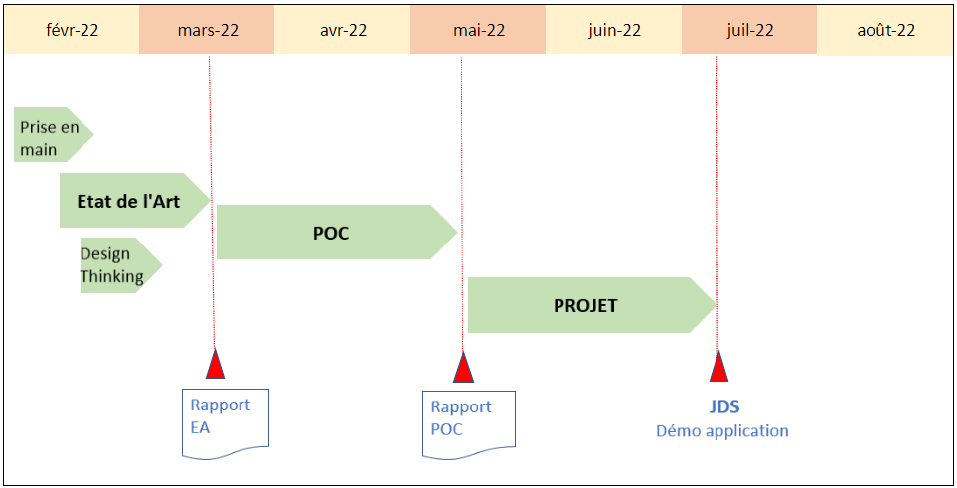
\includegraphics[width=\textwidth]{Planning.png}    
    \caption{Planning prévisionnel du projet FYW.}
    \label{fig:Planning}
  \end{figure}  
  
  J'ai réalisé ce projet dans une équipe de 11 stagiaires, tous en stage de fin d'études. Étant donné les multiples parties concernant le projet, 
  à savoir la détection d'objets, la localisation de l'utilisateur et la gestion des interactions vocales, nous avons dû nous séparer en 3 
  groupes afin de réaliser les états de l'art et les preuves de concept. J'ai personnellement travaillé sur la partie s'intéressant à la 
  localisation et le guidage de l'utilisateur dans son environnement. 
  \pagebreak
 
  \section{État de l'art (8 à 10 p)}  
  \subsection{Recherches bibliographiques}
  % TODO: Modifier le nombre d'articles si j'en résume moins. Pour le moment j'ai écrit "8".
  Dans cette section je présente les recherches bibliographiques que j'ai pu effectuer avec mon groupe lors de la phase d'état de l'art.
  Cet état de l'art concerne la partie de localisation et de guidage de l'utilisateur. 8 publications ont été retenues, nous les avons 
  confrontées et comparées afin de n'en sélectionner qu'une sur laquelle nous allions nous concentrer lors de la phase de preuve de 
  concept. 

  \subsubsection{Wearable Travel Aid for Environment Perception and Navigation of
  Visually Impaired People}

  L'appareil consiste en une caméra grand public rouge, vert, bleu avec de la profondeur (RGB-D pour red, green, blue, depth)
  et une unité de mesure inertielle (IMU pour Inertial Measurement Unit), c'est un capteur qui consiste généralement en des gyroscopes 
  pour mesurer des vitesses angulaires et des accéléromètres pour mesurer la force. Ces appareils sont montés sur une paire de lunettes
  et reliés à un téléphone. L'appareil proposé dans cette solution se sert de la continuité de la hauteur du sol entre les images 
  adjacentes pour segmenter le sol avec précision et rapidité pour ensuite chercher la direction du mouvement en fonction du sol.
  Un réseau de neurones à convolution (CNN pour Convolutional Neural Network) léger est utilisé pour la reconnaissance d'objets 
  (PeelNet avec l'ensemble de données "MS COCO" contenant des images de dimensions 640 x 640). Son schéma de fonctionnement est présenté 
  dans la figure \ref{fig:ReconnaissanceP1}. Il permet de récupérer des informations concernant les endroits aux alentours et l'orientation 
  des objets environnants. Le schéma de fonctionnement du système est présenté dans la Figure \ref{fig:PipelineP1}.

  \begin{figure}[hbt]  
    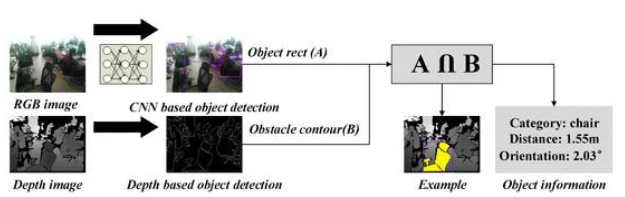
\includegraphics[width=\textwidth]{RecognitionP1.png}    
    \caption{Schéma présentant le fonctionnement du système de reconnaissance d'objets.}
    \label{fig:ReconnaissanceP1}
  \end{figure} 

  \begin{figure}[hbt]  
    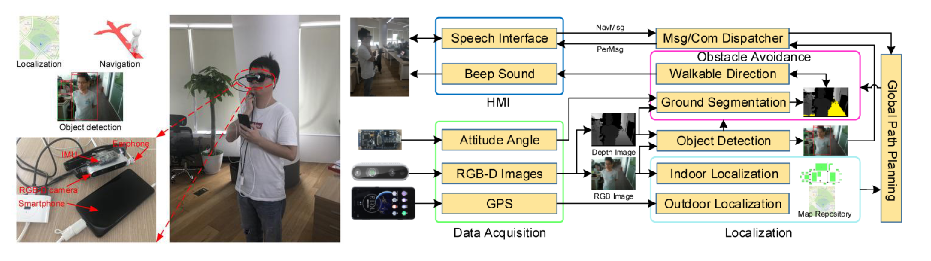
\includegraphics[width=\textwidth]{PipelineP1.png}    
    \caption{Schéma de fonctionnement du système proposé.}
    \label{fig:PipelineP1}
  \end{figure} 

  Le système de navigation contient un module de localisation intérieur qui va nous intéresser: un algorithme VSLAM (Visual Simultaneous 
  Localization and Mapping) est utilisé. SLAM est un problème de computer vision visant à traquer les mouvements d'un module en se basant
  sur ce qu'il voit. Il faut traiter les objets dynamiques qui entrent et sortent du champ de vision pour ne pas les prendre en computer
  dans l'estimation de la position du module. L'estimation se fait en trouvant des points clés sur les images successives.  Visual SLAM
  se sert des informations récuperées pour trianguler la position 3D du module. 
  
  \pagebreak

  \subsubsection{CDSFusion: Dense Semantic SLAM for Indoor Environment Using CPU
  Computing}  

  La solution CDSFusion se sert d'images RGB comme l'article précédent ainsi qu'un capteur IMU comme paramètres d'entrée et est composée de 
  3 modules imagés dans la Figure \ref{fig:PipelineP2}:

  \paragraph{Le module VIO}
  Le module d'odométrie visuelle-innertielle (VIO pour Visual-Inertial Odometry) se sert des entrées pour estimer avec précision la position 
  afin de proposer une trajectoire. Ce module VIO est basé sur VINS-Mono. VINS-Mono est un framework SLAM en temps réel pour les 
  systèmes visuo-inertiels monoculaires. Il utilise une méthode de fenêtre glissante basée sur des optimisations pour fournir une odométrie 
  visuelle-inertielle de haute précision.
  Les features FAST (Features from accelerated segment test) ont été adaptées pour accélérer le VIO à 
  la place des feature Shi-Thomas (une manière de détecter les coins sur une image) et la profondeur a été introduite afin d'obtenir une échelle 
  plus précise. Les résultats expérimentaux montrent que les features FAST augmentent la rapidité du système d'une manière plus conséquente 
  que les features Shi-Tomas et ORB avec la même précision et robustesse. Ce module est composé de 3 parties:

  \underline{Visual-Inertial Frontend: }
  prend en charge le traitement des données issues des capteurs. Les mesures effectuées par le capteur IMU
  sont préintégrées entre deux images consécutives, le frontend de vision détecte les FAST
  et les traque entre les images consécutives en utilisant l'algorithme KLT optical flow.

  \underline{Back-End:} est utilisé pour fusionner les mesures traitées afin d'obtenir l'estimation de la position. Une optimisation non linéaire
  est utilisée pour relocaliser et optimiser le calcul de la position en fonction de la boucle détectée, en utilisant le solveur Ceres. 

  \underline{Le module de détection de boucle: } permet de relocaliser et optimiser le calcul de la position en fonction de
  la boucle détectée. En effet, une boucle est détectée lorsque l'on a réalisé une boucle dans le parcours d'un chemin, il devient alors inutile
  de recalculer la position tant que l'utilisateur se situe dans cette boucle, on peut alors facilement optimiser le calcul de la position en se 
  basant sur des calculs précédemment effectués. Cela se base sur la bibliothèque DBoW2 qui est à l'état de l'art de la reconnaissance d'endroits 
  par sac de mots (bag of words approach). De même, lorsqu'une boucle est détectée, une optimisation est possible pour le calcul de la position 
  globale. Cette optimisation est similaire à la méthode VINS-Mono.

  \paragraph{Le module de segmentation sémantique}
  La segmentation sémantique résulte d'images RGB en entrée qui sont acquises en temps réel en utilisant le module de segmentation PSPNet. 
  Le module de segmentation sémantique traite chaque image RGB et retourne des vecteurs indiquant la probabilité d'appartenance à une classe
  pour chaque pixel. Ils classifient et colorent chaque pixel en fonction de la plus haute probabilité d'appartenance à une classe. 
  L'image segmentée finale est composée des pixels colorés et est transmise au module de reconstruction 3D.

  \paragraph{Le module de reconstruction 3D}

  Le nuage sémantique local est généré en utilisant une image sémantique (générée par le module précédent) et une carte de profondeur. 
  Ce nuage local servira à produire un nuage global une fois qu'il sera combiné avec les estimations de position de la caméra depuis le module VIO.
  Pour construire une carte 3D globale qui soit précise, un modèle basé sur des voxels est utilisé pour filtrer le bruit et extraire un mesh global.
  À chaque image importante (Keyframe), la carte de profondeur courante est transformée en nuage de points 3D, ensuite les options Voxblox et FAST
  sont adaptées, le nuage local de points 3D est transformé en mesh local et ensuite ce mesh local est intégré dans le mesh global. L'ensemble de 
  cette procédure est réalisée en temps réel sur CPU. Voxblox est une bibliothèque de cartographie volumétrique basée principalement 
  sur les TSDF (Truncated Signed Distance Fields).

  \begin{figure}[hbt]  
    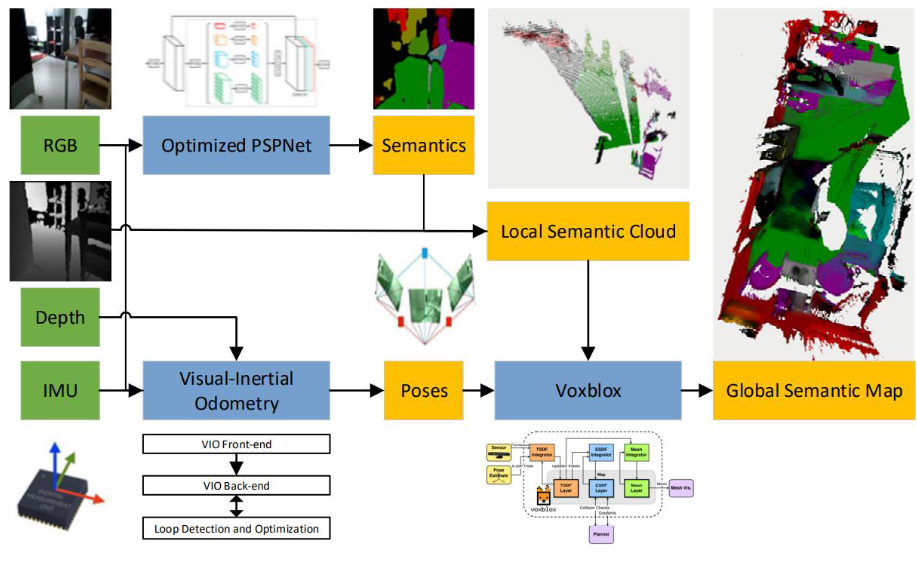
\includegraphics[width=\textwidth]{PipelineP2.png}    
    \caption{Schéma présentant le fonctionnement du système proposé.}
    \label{fig:PipelineP2}
  \end{figure} 
  
  \pagebreak  

  \subsubsection{Towards Real-time Semantic RGB-D SLAM in Dynamic Environments} 

  Cet article présente une méthode de SLAM s'inspirant des features ORB (Oriented FAST and Rotated Brief).
  Le module de segmentation sémantique est une adaptation de SegNet, un réseau de neurones léger qui permet un traitement en temps réel.
  La segmentation se concentre sur des objets dynamiques dont les caractéristiques ne seront pas utilisées dans la création de 
  la carte locale. La segmentation est faite uniquement sur les images clés les plus récentes, accélérant grandement le processus.
  La segmentation peut être très rapide, mais reconnaît principalement les objets qu'elle connaît déjà et est moins efficace dans des 
  milieux inconnus avec des objets dynamiques nouveaux. Ce module essaye de résoudre ce problème.
  Pour chaque nouvelle image l'idée est d'utiliser l'algorithme du K-means pour segmenter l'image de profondeur en N clusters.
  Chaque cluster est considéré comme faisant partie du même objet. Pour chaque cluster, une erreur de reprojection est calculée. Si une 
  des erreurs moyennes est relativement supérieure aux autres, le cluster est considéré comme un objet dynamique et les points caractéristiques
  de l'objet seront supprimés du traitement. Cette manière de traiter les images permet de réduire le taux de faux positifs. 
  Les comparaisons sont effectuées d'une image clé à une autre puisqu'elles se ressemblent beaucoup, mais aussi entre la première estimation
  et les cartes locales obtenues.

  \pagebreak
  % TODO: Prendre l'explication d'ORB SLAM2 et insérer l'ajout d'ORB SLAM 3.

  \subsubsection{ORB-SLAM3: An Accurate Open-Source Library for Visual, Visual-
  Inertial and Multi-Map SLAM}

  \pagebreak

  \subsubsection{A Wearable Navigation Device for Visually Impaired People Based on
  the Real-Time Semantic Visual SLAM System}


  \pagebreak
  
  \subsubsection{DGS-SLAM A Fast and Robust RGBD SLAM in Dynamic Environments
  Combined by Geometric and Semantic Information}

  \pagebreak


  \subsection{Synthèse}

  \pagebreak

  \subsection{Conclusion}

  \pagebreak
  \section{Les dimensions techniques du projet (8 à 12 p)}
  Description des objectifs/tâches qui vous ont été confiés, votre réussite ou votre contribution à
  l’atteinte des objectifs collectifs. Vous exposerez les difficultés rencontrées et la manière dont vous
  les avez abordées. Vous mettrez également en valeur l’originalité éventuelle de votre approche, les
  choix et décisions que vous aurez prises. Vous mettrez vos travaux et réalisations en perspective par
  rapport à l’ensemble du projet et son historique.

  \pagebreak
  \section{Les dimensions humaines et managériales (3 à 5 p)}
  Les dimensions humaines et managériales internes à l’organisme d’accueil. Cette partie consiste en
  une présentation analytique des processus d’entreprise. Selon les cas, elle portera sur la conduite de
  projet, les aspects organisationnels, la gestion du changement, le travail en groupe, l’énoncé des
  objectifs individuels et de l’équipe, la contribution à l’atteinte des objectifs, les difficultés rencontrées,
  les aides reçues, etc. Les difficultés propres à l’entreprise ou au service dans lequel la mission a été
  effectuée doivent être abordées de façon professionnelle pour que le jury ait une appréciation réaliste
  des conditions du travail réalisé.  

  \pagebreak
  \section{Conclusion (2 à 3 p)}
  La conclusion générale, de quelques pages, porte sur l’ensemble de votre expérience technique et
  humaine. Une première partie correspond au bilan et une deuxième partie expose les possibilités
  d’évolution du projet, du produit. Enfin, vous présenterez vos perspectives d’évolution par rapport à
  votre projet professionnel initial. Vous préciserez les compétences que vous avez développées en
  école d’ingénieurs et durant votre mission de fin d’études et préciserez vos axes d’amélioration.

  \pagebreak
  \section{Bibliographie}
  Les sources extérieures sont bienvenues à condition d’être citées avec précision et mentionnées dans
  une annexe bibliographique au rapport et d’être multiples et diversifiées.
  Ces sources doivent être clairement renvoyées aux éléments numérotés de la bibliographie.

  \pagebreak
  \section{Annexes}
  - Glossaires des termes techniques, notions fondamentales rappelées simplement, \\
  - Code informatique, éventuellement utile pour démontrer la réalité des livraisons, \\
  - Détails sur le contexte ou sur la structure d’accueil. 

\end{document}